\documentclass[lithuanian,a4paper,12pt]{article}
\usepackage{babel}
\babelfont{rm}{FreeSerif}
% \usepackage[T1]{fontenc} % Don't need this when using LuaLatex instead of PDFLatex
\usepackage{amsmath}
\usepackage{graphicx}
\usepackage{float}
\usepackage{minted}
\usemintedstyle{vs}
\usepackage{hyperref}
\usepackage{csquotes}

\newcommand{\mil}{\mintinline{python}}

\title{Vienmatis optimizavimas}
\author{Kristupas Dansevičius}
\date{\today}

\begin{document}
\maketitle
\tableofcontents

\section{Įvadas}
Šis laboratorinis darbas atsiskaitomas optimizavimo metodų kurse Vilniaus Universitete. 
Šiame darbe nagrinėjami trys vienmačio optimizavimo metodai:
intervalo dalijimo pusiau metodas, auksinio pjūvio metodas ir Niutono metodas. 

\section{Užduotis}
1-ojo laboratorinio darbo (iš viso yra 4 per semestrą) užduoties reikalavimai:
\begin{enumerate}
    \item Suprogramuoti šiuos metodus (naudota Python programavimo kalba)
    \item Aprašyti duotąją \textbf{tikslo funkciją} - tai funkcija, pagal kurią yra optimizuojama naudojant minėtus metodus, t.y., ieškomas jos \textbf{lokalus minimumas}, kuris ir bus ir \textbf{globalusis minimumas}. Taip yra todėl, kad funkcija nurodytam intervale yra \textbf{iškiloji}: tarp bet kurių dviejų funkcijos taškų nubrėžus liniją, visos funkcijos reikšmės yra žemiau šios linijos. Kitaip pasakius, funkcijoje nėra jokių ``duobių'', į kurias optimizuojant galima patekti ir ``užstrigti'', kurios būtų tik lokalūs, bet ne globalūs minimumai. Pagal reikalavimus (pritaikius studento numerio porą skaitmenų), duotoji tikslo funkcija yra:
        \begin{equation}
            f(x) = \frac{(x^2 - 5)^2}{4}
        \end{equation}
    \item Minimizuoti funkciją intervalo metodais - intervalo dalijimo pusiau ir auksinio pjūvio - naudojant intervalą $[0,10]$ iki tikslumo $10^{-4}$ bei Niutono metodu nuo $x_0 = 5$ kol žingsnio ilgis (Lipschitzo konstanta / tolerancija) didesnis už $10^{-4}$
    \item Palyginti rezultatus: gauti sprendiniai, rastas funkcijos minimumo įvertis (taško, kuriame funkcija turi mažiausią reikšmę), atliktų žingsnių (iteracijų) ir funkcijų skaičiavimų skaičius (tikslo funkcijos ``iškvietimų'' programoje)
    \item Vizualizuoti tikslo funkciją ir bandymo taškus (kuriuose paskaičiuota tikslo funkcija ir buvo naudojami algoritme)
\end{enumerate}

\section{Tikslo funkcijos aprašymas}
Pateikiamas programoje aprašytos tikslo funkcijos kodas, naudojantis Python objektinio programavimo galimybėmis, panaudojant \mil{class}. Šioje tikslo funkcijos klasės aprašyme yra sekamas tikslo funkcijos iškvietimų kiekis, iškvietimus vykdant iš suprogramuotų optimizavimų metodų kodo. Pasak \url{https://www.sympy.org/scipy-2017-codegen-tutorial/notebooks/22-lambdify.html}, \textquote{Behind the scenes \mil{lambdify} constructs a string representation of the Python code and uses Python's \mil{eval} function to compile the function.} Klasėje yra saugoma simbolinės išraiškos (\url{https://en.wikipedia.org/wiki/S-expression}) ne tik pačios tikslo funkcijos, bet ir jos pirmos ir antros eilės išvestinių.

\pagebreak
\begin{minted}{python}
class ObjectiveFunction:
    def __init__(self) -> None:
        self.calls = 0

        self.x: sp.Symbol = sp.symbols('x')
        self.expr: sp.Expr = (self.x**2 - 5)**2 / 4 # type: ignore

        self.expr_prime: sp.Expr = sp.diff(self.expr, self.x)
        self.expr_double_prime: sp.Expr = sp.diff(self.expr, self.x, 2)

        self.f = sp.lambdify(self.x, self.expr, 'numpy')
        self.df = sp.lambdify(self.x, self.expr_prime, 'numpy')
        self.ddf = sp.lambdify(self.x, self.expr_double_prime, 'numpy')

    def __call__(self, x: float) -> float:
        self.calls += 1
        return self.f(x)
    
    def first_derivative(self, x:float) -> float:
        self.calls += 1
        return self.df(x)
    
    def second_derivative(self, x:float) -> float:
        self.calls += 1
        return self.ddf(x)
    
    def print_symbolic(self):
        print("f(x) =", self.expr)
        print("f'(x) =", self.expr_prime)
        print("f''(x) =", self.expr_double_prime)
    
    def reset(self):
        self.calls = 0
\end{minted}

\section{Metodai}
\subsection{Intervalo dalijimo pusiau metodas}
Tai tritaškis intervalo dalijimo pusiau metodas (t.y., kiekvienai optimizavimo algoritmo iteracijai naudojami 3 taškai), kurio principas yra itin paprastas. Intervale \mil{[left_bound, right_bound]}, kurio ilgis \mil{interval_length = right_bound - left_bound}, panaudojami 3 taškai:
\begin{itemize}
    \item \mil{x_middle} - vidurinis taškas esantis intervalo viduryje, \mil{x_{middle} = (left_bound + b) / 2}
    \item \mil{x_1} - tarp kairiojo intervalo krašto \mil{left_bound} ir vidurinio taško \mil{x_middle} esantis taškas, \mil{x_1 = (b - a) * 0.25}
    \item \mil{x_2} - analogiškai kaip \mil{x_1}, tik kitoje intervalo pusėje tarp \mil{x_middle} ir \mil{right_bound} esantis taškas, \mil{x_2 = (b - a) * 0.75}
\end{itemize}

\subsection{Auksinio pjūvio metodas}
Trumpas metodo aprašymas.

\subsection{Niutono metodas}
Trumpas metodo aprašymas.

\section{Rezultatai}
Gauti šie rezultatai:

\begin{itemize}
    \item Intervalo dalijimo pusiau metodas: 
        $x_{\min} \approx 2.236$, iteracijų: 17, funkcijos iškvietimų: 28
    \item Auksinio pjūvio metodas:
        $x_{\min} \approx 2.236$, iteracijų: 24, funkcijos iškvietimų: 26
    \item Niutono metodas:
        $x_{\min} \approx 2.236$, iteracijų: 6, funkcijos iškvietimų: 12
\end{itemize}

\section{Vizualizacija}
Žemiau pateikiamos tikslo funkcijos ir taikytų metodų vizualizacijos.

\begin{figure}[H]
    \centering
    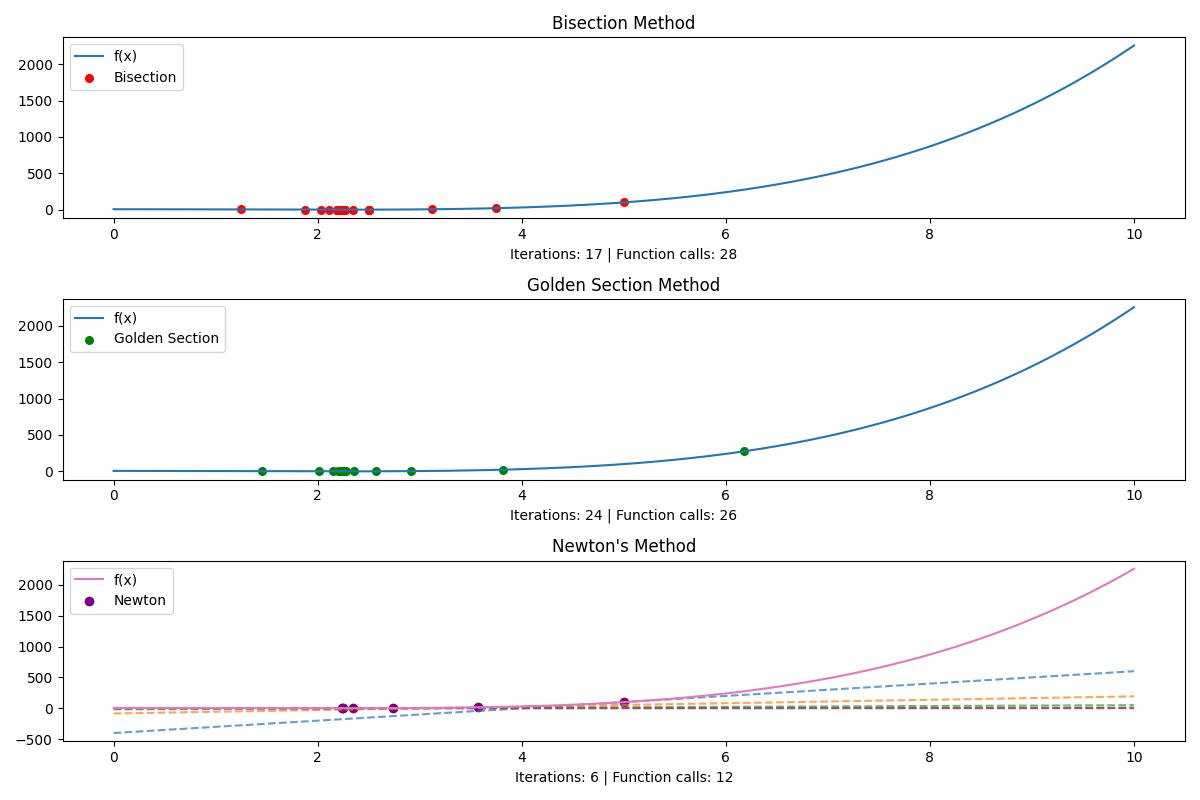
\includegraphics[width=\textwidth,height=10cm]{figure-1.jpeg}
    \caption{\label{fig:all}Funkcijos $f(x)$ optimizavimo vizualizacija.}
\end{figure}

\section{Išvados}
\begin{itemize}
    \item Visi metodai rado minimumą ties $x \approx \sqrt{5}$.
    \item Intervalo metodai (intervalo dalijimo pusiau ir auksinio pjūvio) reikalauja daugiau iteracijų ir tikslo funkcijos iškvietimų, bet yra paprastesni.
    \item Su naudotais parametrais (tikslo funkcija / intervalu / tikslumu) auksinio pjūvio optimizavimo efektyvumo pranašumas prieš intervalo dalijimo pusiau optimizavimo metodą pagal tikslo funkcijos kvietimų kiekį neišryškėjo
\end{itemize}

\section{Kodas}
\inputminted{python}{../code/main.py}
\section{Šaltiniai}

1. Python paketo \mintinline{python}{sympy} oficialaus puslapio 2017-ųjų metų užrašų tipo mokymo programa / tutorial \url{https://www.sympy.org/scipy-2017-codegen-tutorial/notebooks/22-lambdify.html}
\end{document}